\chapter{Speech and the sound system}\label{ch:sound}

\epigraph{My mother's mouth opens --\\
one sound pulls out another\\
like winter scarves from a drawer\\
until the whole language\\
tumbles between us.}{}

\section{Introduction}

As English language teachers, we often focus on grammar and vocabulary, along with reading, writing, listening, and speaking. Underpinning all of these, though, is a fundamental aspect of language: \is{pronunciation|(}pronunciation. This chapter introduces English \is{speech production|(}speech and its sound system, providing you with the knowledge and tools to effectively teach reading, listening, and pronunciation to your students.

We'll begin by exploring the complexity of speech production, from the precise control of breathing to the intricate coordination of articulators. Then, we'll examine the sound system of English, considering \is{phoneme|(}phonemes, \is{allophone|(}allophones, and the challenges they present for learners. We'll discuss:

\begin{itemize}[noitemsep]
    \item Setting realistic pronunciation goals for learners
    \item The distinction between phonemes and allophones
    \item Vowel length and quality
    \item \is{syllable!structure|(}Syllable structure and \is{phonotactics|(}phonotactics
    \item \is{suprasegmental|(}Suprasegmental features like \is{stress|(}stress, \is{intonation|(}intonation, and \is{rhythm|(}rhythm
    \item \is{connected speech|(}Connected speech processes
\end{itemize}

\section{Speech production}
Speaking is one of the most complicated things we do. Even when we put aside all the linguistic processing that's completely invisible, the physical act of speech itself remains a feat of remarkable intricacy.

Start with the breath. As we speak, we push an exquisitely controlled stream of air from our lungs, up our windpipe, past our vocal chords, and then out, through the mouth, the nose, or both. This is surprising. While breathing typically occurs automatically, speaking requires voluntary control over the \is{breath control|(}breathing apparatus. Speakers often inhale quickly and deeply, and exhale more slowly to prolong phonation (making speech sounds). This pattern is crucial for long sentences or when emphasis is needed on particular words or phrases.

The muscles of the trunk, which include the abdominal and back muscles, play a supporting role in breathing and speech. These muscles help regulate the pressure within the abdominal and thoracic cavities, enhancing control over the air expelled during speech. There's a feedback loop between trunk stability and breath control.\is{breath control|)}

But what of the mouth, the tongue, the lips, the jaw, the soft palate? The level of precision they achieve rivals that of a fine orchestra, the placement of each articulator shaping the fundamental frequencies and various overtones that characterize the various vowels and consonants. 

The brain has to send signals to each of these structures in a precise sequence and timing. Due to the varying distances between the brain and the different articulators, the neural impulses need careful orchestration. Speech production isn't a simple sequence of brain signals matching the order of sounds. The brain issues motor commands in complex patterns that may not follow the phonological order of words, constantly adjusting for varying articulator positions in different sound contexts \citep[108]{Tatham2006speech}.

\subsection{Articulatory organs and their roles}

\is{articulatory organs|(}Speech production involves a coordinated effort of several organs, each contributing to the formation of sounds. Figure \ref{fig:articulation} illustrates various \is{place of articulation|(}places of articulation, which we'll explore in this section.

\begin{figure}
    \centering
    
\includegraphics[width=0.5\linewidth]{figures/Places_of_articulation.svg.png}
    \caption{Passive and active places of articulation: (1 \& 2) Labial; (3) Dental; (4) Alveolar; (7) Palatal; (8) Velar; (9) Uvular; (11) Glottal. By User:ish shwar (original .png deleted), .svg by Rohieb, \href{http://creativecommons.org/licenses/by-sa/3.0/}{CC BY-SA 3.0}, via Wikimedia Commons}
    \label{fig:articulation}
\end{figure}

A \textsc{place of articulation} is a location in the vocal tract where the tongue, lips, or other organ can form a constriction or closure to produce a speech sound. We'll focus on those most relevant to English.

\paragraph*{Lungs} The lungs provide the airstream for most speech sounds. During speech, we control this airflow, using it to generate different sounds as it passes through the vocal tract.

\paragraph*{Larynx and vocal folds (11)} The \is{larynx}larynx houses the \is{vocal folds (cords)|(}vocal folds. When these folds vibrate as air passes through, they produce \is{voicing|(}voicing, forming vowels and voiced consonants like /b/, /d/, /g/, /n/, /m/, /r/, and /l/. Holding the folds apart results in voiceless sounds like /p/, /t/, and /k/.

\paragraph*{Glottis (11)} The space between the vocal folds is called the glottis. When the vocal folds are brought together abruptly, they produce a \is{glottal stop}glottal stop, heard in expressions like \textit{uh-oh} and other words in various dialects.

\paragraph*{Velum (8)} The \is{velum (soft palate)|(}velum (soft palate) controls \is{nasal!velum, role in}nasal airflow. A lowered velum creates \is{nasal!sounds}nasal sounds like /m/, /n/, and /ŋ/ (the $\langle$ng$\rangle$ in \textit{sing}), while a raised velum produces oral sounds. (Try saying \textit{murmur} or \textit{nanny} while firmly holding your nose.) The velum also serves as a place of articulation for \is{velar!sounds}velar consonants such as /k/, /g/, and /ŋ/.\is{velum (soft palate)|)}

\paragraph*{Uvula (9)} Some languages use the \is{uvular}uvula as a place of articulation. This is uncommon in English, though it occurs in some dialects. An example of a uvular sound is the French\il{French} /ʁ/ in \textit{rouge}.


\paragraph*{Teeth (3) and alveolar ridge (4)} These serve as points of contact for the tongue for many sounds, including /t/, /d/, /s/, and /z/.

\paragraph*{Tongue} The \is{tongue!parts of (tip, blade, front, back)}tongue's versatility allows for a wide range of sound productions:
\begin{itemize}[noitemsep]
    \item \textit{Tip (17) and blade (16)}: For \is{alveolar!sounds}alveolar sounds like /t/, /d/, /s/, and /z/.
    \item \textit{Front (15)}: For \is{palatal!sounds}palatal sounds like /ʃ/ (the $\langle$sh$\rangle$ in \textit{ship}).
    \item \textit{Back (14)}: For velar sounds like /k/ and /g/.
\end{itemize}

\paragraph*{Lips (2)} The lips shape sounds in various ways:
\begin{itemize}[noitemsep]
    \item Rounded: As in /u/ (the vowel sound in \textit{boot})
    \item Spread: As in /i/ (the vowel sound in \textit{beet})
    \item Brought together: For \is{bilabial}bilabial sounds like /p/ and /b/
\end{itemize}
\is{articulatory organs|)}\is{place of articulation|)}\is{speech production|)}

\section{The sound system}
English pronunciation varies from place to place and time to time. These is no universal standard, so I will describe the English that I speak, a somewhat conservative variety found in and around Toronto. When I say conservative, I mean that I don't have a number of the sound changes that many folks I grew up with. When I say \textit{which}, for instance, it doesn't sound like \textit{witch}: it starts /hw/, not /w/. 

I can't emphasize enough that there is no single correct pronunciation. There is no way to adjudicate between those who say /ˈɑftən/ and those who say /ˈɑfən/, those who say /ˈnu.kli.ɚ/ and those who say /ˈnju.kli.ɚ/ or /ˈnu.kjə.lɚ/, those who apologize with /ˈsɑɹ.i/ and those who use /ˈsɔɹ.i/, etc. Even if you've never learned the \is{International Phonetic Alphabet (IPA)}international phonetic alphabet (IPA), I expect you can work out that those words are \textit{often}, \textit{nuclear}, and \textit{sorry}. 

But it's time to go through the symbols of the International Phonetic Alphabet (IPA) one by one. Most of these are just what you'd expect: /m/ as in \textit{mom}, /d/ as in \textit{dad}, etc. Only a few are unfamiliar (/ð/, /ʒ/, /d͡ʒ/, /ŋ/, /θ/, /ʃ/, \& /t͡ʃ/) or confusing (/j/ is the ``y sound" in \textit{yellow}).

\subsection{Consonants}

I have roughly 24 \textsc{consonant} \is{consonant!phonemes, number of}phonemes in my dialect (depending on whether you count things like the glottal stop in \textit{uh-oh}), each characterized by its place and manner of articulation, and voicing. Let's explore these features:

\subsubsection{Place of Articulation}

The place of articulation refers to where in the vocal tract the airflow is obstructed. English uses these main places:

\begin{itemize}[noitemsep]
    \item \textit{Bilabial} (2): Both lips come together. Examples: /p/, /b/, /m/, \& /w/
    \item \textit{Labiodental} (2 \& 3): Lower lip touches upper teeth. Examples: /f/ \& /v/
    \item \textit{Dental} (3): Tongue tip behind or between teeth. Examples: /θ/ (as in \textit{thin}), /ð/ (as in \textit{this})
    \item \textit{Alveolar} (4): Tongue tip or blade on the \is{alveolar!ridge}alveolar ridge. Examples: /t/, /d/, /s/, /z/, /n/, \& /l/
    \item \textit{Post-alveolar} (5): Tongue blade behind the alveolar ridge. Examples: /r/, /ʃ/ (as in \textit{ship}), /ʒ/ (as in \textit{measure}), /t͡ʃ/ (as in \textit{chip}), \& /d͡ʒ/ (as in \textit{judge}). Here, /t͡ʃ/ and /d͡ʒ/ are single phonemes, even though they're represented in the IPA with two symbols each.
    \item \textit{Palatal} (7): Tongue body against the hard palate. Example: /j/ (as in \textit{yes})
    \item \textit{Velar} (8): Tongue body against the soft palate. Examples: /k/, /g/, \& /ŋ/ (as in \textit{sing})
    \item \textit{Glottal} (11): Constriction at the vocal folds. Example: /h/
\end{itemize}

\subsubsection{Manner of Articulation}

The \textsc{\is{manner of articulation}manner of articulation} describes how the airflow is obstructed. English uses these manners:

\begin{itemize}[noitemsep]
    \item \textit{Plosives} (also called \textit{stops}): Complete closure followed by sudden release. Examples: /p/, /b/, /t/, /d/, /k/, \& /g/
    \item \textit{Nasals}: Velum lowered, air escapes through nose. Examples: /m/, /n/, \& /ŋ/
    \item \textit{Fricatives}: Close approximation of articulators, turbulent airflow. Examples: /f/, /v/, /θ/, /ð/, /s/, /z/, /ʃ/, /ʒ/, \& /h/
    \item \textit{Affricates}: A \is{plosive (stop)}plosive beginning and a \is{fricative}fricative end. Examples: /t͡ʃ/ \& /d͡ʒ/
    \item \textit{Approximants}: Articulators approach each other but don't cause turbulence. Examples: /r/, /j/, \& /w/
    \item \textit{Lateral}: Air escapes around sides of tongue. Example: /l/
\end{itemize}

\subsubsection{Voicing}

\textsc{Voicing} refers to whether the vocal folds vibrate during the production of a sound. English consonants come in voiced-voiceless pairs for many places and manners of articulation:

\begin{itemize}[noitemsep]
    \item \textit{Voiced}: /b/, /d/, /g/, /v/, /ð/, /z/, /ʒ/, /d͡ʒ/, /m/, /n/, /ŋ/, /l/, /r/, /j/, \& /w/
    \item \textit{Voiceless}: /p/, /t/, /k/, /f/, /θ/, /s/, /ʃ/, /t͡ʃ/, \& /h/
\end{itemize}

Understanding these features helps in identifying why certain sounds might be challenging for learners. For instance, a native speaker of a language without the /θ/ sound might substitute it with /s/ or /t/, as these are the closest sounds in their phonetic inventory.

\subsection{Vowels}

My dialect has about nine main \is{vowel!phonemes, number of}vowel phonemes and seven diphthongs. \textsc{Vowels} are characterized by the position of the \is{tongue!position, for vowels}tongue, the shape of the lips, and their length. The vowels in my dialect are shown in Figure \ref{fig:Toronto-vowels}.

\begin{figure}
\begin{center}
\begin{tikzpicture}[scale=5]
  % Draw the vowel trapezoid
  \draw (0.42,0) -- (0.9,0) -- (0.9,1) -- (0,1) -- cycle;
  \draw (0.66,0) -- (0.45,1);
  \draw (0.28,0.3333) -- (0.9,0.3333);
  \draw (0.14,0.6666) -- (0.9,0.6666);


  % Place vowel symbols at appropriate positions
  % Close vowels
  \node at (0.1, 0.95) {i};
  \node at (0.6, 0.90) {u};
  \node at (0.46, 0.7) {ɪ};
  \node at (0.7, 0.72) {\textupsilon};
  

  % Mid vowels
  \node at (0.46, 0.36) {\textepsilon}; 
  \node at (0.56, 0.5) {\textschwa}; 
  \node at (0.2, 0.6) {e};
  \node at (0.8, 0.58) {o};

  % Open vowels
  \node at (0.55, 0.05) {æ};
  \node at (0.85, 0.1) {\textscripta}; 
  \node at (0.44, 0.03) {a}; 
  \node at (0.65, 0.3) {ʌ};
  \node at (0.75, 0.4) {ɔ};
\end{tikzpicture}
\end{center}




    \caption{Vowel chart of Canadian English. This diagram represents the position of the tongue in the mouth for selected vowels. The horizontal axis shows tongue position from front (left) to back (right), while the vertical axis represents tongue height from close/high (top) to open/low (bottom).}
    \label{fig:Toronto-vowels}
\end{figure}
%Figure 7.2 shows the place of articulation of /ɒ/, which I don't list as among the phoneme repertory; but not that of /ɑ/, which I do; or those of /a/ or /e/, which I also do (as diphthong ingredients).

\subsubsection{Tongue Position}

The tongue position is described in terms of height (high, mid, low) and frontness (front, central, back).

\begin{figure}
    \centering
    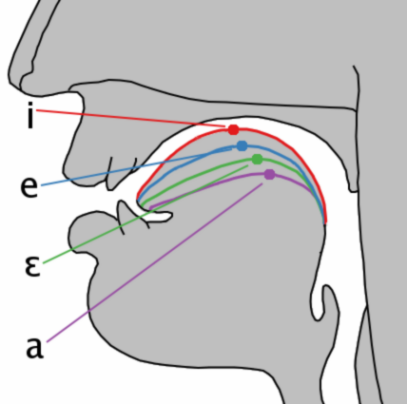
\includegraphics[width=0.25\linewidth]{figures/Cardinal_vowel_tongue_position-front.png}
    \caption{Cross-section of the mouth showing tongue positions for selected vowels. The diagram illustrates how the tongue's height and frontness in the mouth correspond to different vowel sounds. \\\hfill By Ishwar \href{http://creativecommons.org/licenses/by-sa/3.0/}{CC BY-SA 3.0}, via Wikimedia Commons.}
    \label{fig:cardinal-vowels}
\end{figure}

\begin{itemize}[noitemsep]
    \item \textit{High front}: /i/ (as in \textit{beet}), /ɪ/ (as in \textit{bit})
    \item \textit{High back}: /u/ (as in \textit{boot}), /ʊ/ (as in \textit{book})
    \item \textit{Mid front}: /ɛ/ (as in \textit{bet})
    \item \textit{Mid central}: /ə/ (as in the first syllable of \textit{about})
    \item \textit{Mid back}: /ʌ/ (as in \textit{but})
    \item \textit{Low front}: /æ/ (as in \textit{bat})
    \item \textit{Low back}: /ɑ/ (as in \textit{bot})
\end{itemize}

\subsubsection{Lip Rounding}

Vowels can be rounded or unrounded:

\begin{itemize}[noitemsep]
    \item \textit{Rounded}: /u/, /ʊ/, /o/
    \item \textit{Unrounded}: All others
\end{itemize}

\subsubsection{Diphthongs}

\textsc{\is{diphthong|(}Diphthongs} are vowel sounds that involve a change in quality during their production (from Greek \textit{diphthongos} `having two sounds'). For example, \textit{ride} starts at /a/ and ``glides'' to /ɪ/. My dialect includes the following diphthongs.

\begin{itemize}[noitemsep]
    \item /aɪ/ (as in \textit{ride} before voiced consonants)
    \item /ʌɪ/ (as in \textit{write} before voiceless consonants)
    \item /aʊ/ (as in \textit{loud} before voiced consonants)
    \item /ʌʊ/ (as in \textit{out} before voiceless consonants)
    \item /ɔɪ/ (as in \textit{boy})
    \item /eɪ/ (as in \textit{bait})
    \item /oʊ/ (as in \textit{boat})
\end{itemize}
\is{diphthong|)}

Many languages have fewer vowel distinctions than English, making vowel production and discrimination a common challenge for learners. For instance, speakers of languages with a five-vowel system (/a/, /e/, /i/, /o/, /u/) may struggle to differentiate between pairs like /i/ \& /ɪ/ or /u/ \& /ʊ/.






\section{Setting pronunciation goals}

When learning a new language, setting realistic and achievable \is{pronunciation!goals|(}pronunciation goals is crucial for both learners and educators. However, determining what constitutes an appropriate pronunciation goal can be a complex and sometimes controversial issue, particularly in the context of English language learning.

One perspective on pronunciation goals is the idea of ``native-like'' pronunciation. From this viewpoint, the ultimate aim of pronunciation instruction is to help learners achieve a level of proficiency that is indistinguishable from that of a native speaker. This goal is often motivated by the belief that \is{accent!native-like vs intelligible}native-like pronunciation is necessary for effective communication and social acceptance within the target language community. It's also the goal that many students have, at least implicitly.

But the concept of native-like pronunciation has been challenged on several grounds. First, the very notion of a ``native speaker'' is very hard to pin down, given the wide variety of \is{accent!regional variation}accents and dialects that exist within any language community, especially in a global language like English. Second, research has shown that even highly proficient English speakers who did not grow up speaking English typically retain some degree of \is{accent!foreign}foreign accent, and that this accent does not necessarily impede communication or social integration \citep{DerwingMunro2009}. Third, the pursuit of native-like pronunciation can be demotivating for learners, as it sets an unrealistic standard that may be difficult or impossible to achieve.

An alternative perspective on pronunciation goals emphasizes \is{intelligibility}intelligibility and \is{comprehensibility}comprehensibility over native-likeness. Intelligibility refers to the extent to which a listener can accurately decode the words and utterances produced by a speaker, while comprehensibility refers to the ease with which a listener can understand the meaning of those utterances \citep{DerwingMunro2015}. From this viewpoint, the primary aim of pronunciation instruction is to help learners develop the skills and strategies needed to communicate effectively and efficiently in the target language, even if their pronunciation retains some non-native characteristics.

Research has provided support for the intelligibility and comprehensibility perspective on pronunciation goals. Studies have shown that even speech with noticeable accents~-- typically we don't notice our own accents or those like them~-- can be highly intelligible and comprehensible, and that factors such as speech rate, fluency, and lexical and grammatical accuracy often play a more significant role in communication success than accent \citep{MunroDerwing1995}. Moreover, a focus on intelligibility and comprehensibility can be more motivating for learners, as it emphasizes the communicative value of their language skills rather than their ability to conform to some idealized native-speaker norm.

Another factor to consider when setting pronunciation goals is the role of \is{accent!and identity}identity and individual differences. For some learners, developing a native-like accent may be an important personal or professional goal, reflecting their desire to fully integrate into the target language community or to project a particular social or cultural identity. For others, retaining some degree of foreign accent may be a way of asserting their linguistic and cultural heritage or of expressing their unique personality and style. Ultimately, the choice of pronunciation goals should be informed by a learner's individual needs, motivations, and contexts of language use.

In setting pronunciation goals, it is also important to consider the potential for \is{accent!bias and discrimination}accent discrimination and bias. Everyday experience shows that non-local accents can sometimes trigger negative stereotypes or prejudices, and this can lead to social, educational, or professional barriers for speakers \citep{LippiGreen2012accent}. While the ultimate solution to this problem is greater linguistic diversity and inclusion, language teachers can both help learners surmount accent bias and urge a greater acceptance of non-native speech.

Ultimately, the key to setting effective pronunciation goals is to strike a balance between aspirational and realistic expectations. While the goal of native-like pronunciation may be appropriate for some learners in some contexts, a more broadly applicable and achievable goal is the development of intelligible, comprehensible, and confident speech that allows learners to communicate successfully in a variety of social and professional settings. By prioritizing these communicative outcomes over a narrow focus on accent reduction, language educators can help learners develop the skills and strategies needed to become effective and empowered users of the English language.\is{pronunciation!goals|)}

\section{Phonemes and Allophones} \label{sec:allophones}

The human capacity for language is remarkable.

Not only can we produce and understand complex sounds, but our brains can also categorize these sounds in ways that create meaning. Those sound categories, the smallest ones, the building blocks of spoken English, are \textsc{phonemes} and \textsc{allophones}.

Now, consider, for a moment, the strawberries in Figure \ref{fig:strawberries}. At first glance, they likely appear red to you, a colour universally associated with ripeness in this fruit. But the wavelength of the light from the berries nowhere near the \textcolor{red}{650nm that we typically perceive as red}. In fact, in most contexts, the same wavelengths would typically appear gray with a tinge of cyan (with a peak close to 490nm). Instead, `red' is a process in your brain that guesses at what you must be percieving, given the cyan background, and then serves that up to your conscious experience. It's an optical illusion, nothing more.

\begin{figure}[ht]
    \centering
    
\includegraphics[width=0.5\textwidth]{figures/strawberries.jpg}
    \caption{Are the strawberries red? Image by Akiyoshi Kitaoka.}
    \label{fig:strawberries}
\end{figure}

\textsc{Phonemes} function in a similar way. They are useful illusions that our brains serve up to our conscious experience, \is{phoneme!as mental category}mental categories used to group similar sounding speech units in particular contexts. They're how we tell \textit{cat} from \textit{cot}, \textit{fan} from \textit{van}, \textit{ducks} from \textit{Doug's}, and \textit{ripe} from \textit{wipe}. They're the smallest sounds that make a difference in a language, the colours of words, the psychological experience of speech atoms.

But, just as the redness of the strawberries in Figure \ref{fig:strawberries} depends on the background colour (cyan), the specific sounds that make up a phoneme can vary depending on the language background of the speaker and the surrounding sounds in a word. Red is a mental category, not a physical property of the world. Similarly, the /m/ phoneme~-- the one at both ends of \textit{mom}~-- is a mental category, not a physical property of the world.

As /m/ illustrates, we write phonemes in between slashes. For instance, the phoneme that starts the word \textit{top} is /t/, and so is the one that comes after /s/ in \textit{stop}. 

Recall that phonemes are the smallest speech sounds \uline{that make a difference in a language}. The /t/ phonemes in \textit{top} and \textit{stop} each have even sonic aspects that distinguish them from one another, but not in a way that makes a difference to English speakers.  These different versions of the same phoneme are called \textsc{allophones}. Allophones are simply different ways to pronounce the same sound, without changing the meaning of a word.

For example, the first /t/ in  \textit{top} is \is{aspiration}aspirated~-- it's accompanied by a puff of air, which we show like this [t\textsuperscript{h}]. The second /t/ in \textit{stop} is not; it's just plain old [t]. [t\textsuperscript{h}] and [t] are allophones of the /t/ phoneme.

If you're sure that those two sounds are, in fact, identical~-- as I did the first time I was told that they were different~-- then you should hold a tissue or a flame in front of your mouth and say the two words. Because the /t/ in \textit{top} is aspirated, the tissue or flame will jump (see Figure \ref{fig:top-stop-flame}), something it won't do for the /t/ in \textit{stop}. Give it a try.

\begin{figure}
    \centering
    
\includegraphics[width=0.4\textwidth]{figures/stop.jpg}
    
\includegraphics[width=0.4\textwidth]{figures/top.jpg}
    \caption{The flame reacts to the aspirated /t/ in \textit{top}, but not to the unaspirated /t/ in \textit{stop}.}
    \label{fig:top-stop-flame}
\end{figure}

If you speak a language such as Hindi/Urdu\il{Hindi|(}\il{Urdu}, then you don't need a flame to perceive this difference. It's obvious to you, because /t\textsuperscript{h}/ and /t/ are different phonemes. They seem as different as /t/ and /d/ do to English speakers or as red and cyan.

So, to review, a phoneme is the smallest language sound that makes a difference in a \strong{particular} language. Phonemes are written in slashes, like /ðɪs/. By contrast, \is{phone!vs phoneme}phones are the smallest language sounds that make a difference in human language, and they're written in brackets, like \ob ðɪs{\cb}. While we're at it, spellings are written like $\langle$this$\rangle$.

%Incidentally, do you any¬where explain how phone differs from allophone?

\begin{tcolorbox}[title=Vowels and consonants] \label{sec:vowels-and-consonants}
    We often say that the English vowels are $\langle$a$\rangle$, $\langle$e$\rangle$, $\langle$i$\rangle$, $\langle$o$\rangle$, $\langle$u$\rangle$, and sometimes $\langle$y$\rangle$. But linguists prefer \textsc{vowel} for phonemes, not for graphemes (individual letters or groups thereof represent a sound like $\langle$t$\rangle$ = /t/ and $\langle$th$\rangle$ = /θ/ are called \textsc{\is{grapheme}graphemes}.) When I use \textsc{vowel}, here, that's what I mean: a phoneme, not a letter/grapheme. Same thing for \textsc{consonant}. So English doesn't have five or six vowels. It's got more than 20, depending on the dialect.
\end{tcolorbox}

Two different phones may make no phonemic difference in one language~-- like [t] and [tʰ] in English~-- while being distinct in another. If you said \textit{stop} with an aspirated [tʰ], it would still be /stɒp/. On the other hand, if you changed a [t] in the Hindi\il{Hindi} word /tɑl/ `rhythm' to [tʰ], it would become /tʰɑl/ `plate'.\is{cross-linguistic influence}

Here, English has one phoneme where Hindi\il{Hindi|)} has two. But cases where English has two for one in another language are also common. Japanese speakers, for instance, somewhat famously perceive both English /r/ and /l/ as one phoneme.

In fact, there are even differences among English dialects. In my Ontario English, the vowels in \textit{cot} and \textit{caught} are the same, but many people perceive \textit{cot} with /ɑ/ and \textit{cought} with /ɔ/. For them, these words are as perceptually distinct as \textit{pin} and \textit{pen} or \textit{ban} and \textit{bun}.

So why does this phoneme/allophone business matter for teachers? For one thing, it helps us understand the nature of pronunciation errors. If a Spanish\il{Spanish} speaker says \textit{berry} instead of \textit{very}, they're not messing up the phonemes~-- they're applying Spanish allophonic rules to English. In Spanish, [b] and [β] are allophones of the same phoneme, with [β] occurring between vowels and sounding to English speakers half-way between a /b/ and a /v/. But in English, /b/ and /v/ can change meaning. Recognizing this can help us give more targeted, meaningful feedback.

It also matters because if students sometimes perceive us as saying the ``clear [l]'' in \textit{love} and other times the ``dark [ɫ]'' in \textit{ball}, but we think they're always hearing only the English /l/, then there's a good deal of possibility for miscommunication.

So as ESL teachers, we need a solid grasp of the phoneme/allophone distinction. We need to know which sound differences are phonemic in English (and thus essential for meaning) and which are allophonic (and thus more flexible). We need this knowledge to prioritize our teaching, to troubleshoot learner difficulties, and to make informed choices about pronunciation models and targets.

Luckily, you don't need to be a trained linguist to develop this kind of phonemic awareness. A good place to start is simply by studying a phonemic chart of English, like the ones provided by the \is{International Phonetic Alphabet (IPA)}International Phonetic Association. Get familiar with the symbols, the articulatory descriptions, and the example words. Train your ear to hear the contrasts through minimal pair activities and transcription practice. 

And crucially, start listening to English with ``phonetic ears''. When you hear a learner's pronunciation error, ask yourself: are they mixing up phonemes, or just using non-native allophones? When you listen to regional accents, try to consider precisely how they vary. When you teach new vocabulary, think about how to highlight the phonemic contrasts and relationships.

\section{Vowel Length and Quality} \label{sec:long-vowels}

One area of confusion for ESL learners and teachers alike is the concept of ``long'' and ``short'' vowels in English. This terminology, while widely used, can be misleading, as it conflates two distinct aspects of vowel sounds: duration and quality.

In everyday language, we often describe the vowel in words like \textit{mate} /meɪt/ as being ``long'' and the vowel in words like \textit{mat} /mæt/ as ``short''. But from a phonological perspective, the primary difference between these vowels is not one of length, but of quality. The two vowels are simply distinct sounds, /eɪ/ vs /æ/. But, generally speaking, they have very similar durations.

That said, vowel duration does play a role in English pronunciation, but in a different way. In many varieties of English, vowels tend to be phonetically longer before voiced consonants than before voiceless consonants.

\begin{tcolorbox}[title=Consonant Voicing]
Consonants in English can be either voiced or voiceless. Voiced consonants involve vibration of the vocal cords during production, while voiceless consonants do not. For example, /b/ is the voiced counterpart to voiceless /p/, /d/ to /t/, and /g/ to /k/. If that's not clear, try putting your finger tips to your throat and alternating between /p/ and /b/. You'll feel the vibrations with /b/.
\end{tcolorbox}

For example, the /æ/ vowel in \textit{mad} /mæd/ is typically slightly longer than the /æ/ in \textit{mat} /mæt/, something we can mark with \ob ː{\cb}~as \ob mæt{\cb}~vs \ob mæːd{\cb}. This is because the vibration of the \is{vocal folds (cords)!and voicing}vocal cords during the production of /d/ allows the vowel to be sustained for a bit longer than before the voiceless /t/.\is{vocal folds (cords)|)}

This durational difference is a phonetic detail, though, not a phonological contrast, at least not in English. It doesn't change the identity of the vowel in the same way that the quality difference between /æ/ and /eɪ/ does. In other words, /æ/ in \textit{mad} and /æ/ in \textit{mat} are allophones of the same phoneme, while /æ/ and /eɪ/ are separate phonemes.

For students who have production difficulty with voiced vs unvoiced distinction after vowels (\textit{ba\uline{g}} vs \textit{ba\uline{ck}}, \textit{hi\uline{d}} vs \textit{hi\uline{t}}, etc.), it is sometimes helpful to try ``holding'' the preceding vowels a bit longer, especially if they speak a language in which \is{vowel!length and quality}vowel length is phonemic, that is where /ti/ and /tiː/ could be different words.

\subsection{The pronunciations of \textit{--\op e\cp s} and \textit{--ed}}

Two of the most common inflectional endings in English are \textit{--\op e\cp s}, used for plural nouns and third-person singular present tense verbs, and \textit{--ed}, used for past tense and past participle forms of regular verbs. Despite their simple spellings, these endings can be pronounced in multiple ways depending on the phonological context in which they appear.

The \textit{--\op e\cp s} ending has three possible pronunciations:

\begin{enumerate}[noitemsep]
    \item /s/ after voiceless consonants (except /s/, /ʃ/, /t͡ʃ/): \\\textit{cats} /kæts/, \textit{books} /bʊks/, \textit{laughs} /læfs/
    \item /z/ after vowels and voiced consonants (except /z/, /ʒ/, /d͡ʒ/): \\\textit{dogs} /dɒɡz/, \textit{rooms} /rumz/, \textit{cars} /kɑrz/
    \item /ɪz/ after \is{sibilant}sibilants (hissing or buzzing sounds) (/s/, /z/, /ʃ/, /ʒ/, /t͡ʃ/, /d͡ʒ/): \textit{buses} /bʌsɪz/, \textit{garages} /ɡærɑʒɪz/, \textit{watches} /wɒt͡ʃɪz/
\end{enumerate}

Similarly, the \textit{--ed} ending has three possible pronunciations:

\begin{enumerate}[noitemsep]
    \item /t/ after voiceless consonants (except /t/): \\\textit{walked} /wɔkt/, \textit{helped} /helpt/, \textit{laughed} /læft/
    \item /d/ after vowels and voiced consonants (except /d/): \\\textit{played} /pleɪd/, \textit{showed} /ʃəʊd/, \textit{loved} /lʌvd/
    \item /ɪd/ after /t/ and /d/: \textit{wanted} /wɒntɪd/, \textit{headed} /hedɪd/, \textit{guarded} /ɡɑ:dɪd/
\end{enumerate}

These pronunciation patterns are not random but rather reflect a process called\is{inflection!pronunciation of -(\textit{e})\textit{s} \& -\textit{ed}} \is{assimilation!progressive}progressive assimilation, where the voicing of the final consonant of the base word influences the voicing of the inflectional ending. In other words, voiceless consonants trigger voiceless pronunciations (/s/ and /t/), while \is{voicing!and inflectional endings}voiced consonants and vowels trigger voiced pronunciations (/z/ and /d/). The /ɪz/ and /ɪd/ pronunciations occur when the base word ends in a sound that is phonetically similar to the inflectional ending, in order to maintain the contrast between the two sounds.

The past tense/participle \textit{--ed} ending often causes problems for students who speak particular languages. Such students default to the /ɪd/ ending, even where /t/ or /d/ would typically be preferred. This usually has to do with limits on what and where consonant clusters are allowed to occur in the first language. These are called \textsc{phonotactic} limits and are the topic of the next section.

\section{Syllable Structure and Phonotactics} \label{sec:phonotactics}

If phonemes are the fundamental sound units of English pronunciation, \textsc{\is{syllable|(}syllables} are the fundamental rhythmic units. Every word is composed of one or more syllables, each with its own internal structure and rules for which sounds can go where. This structure underpins everything from word stress to connected speech processes to pronunciation teaching strategies.

At its most basic, a syllable consists of a vowel sound (the \textsc{\is{nucleus (syllable)}nucleus}), optionally preceded by one or more consonants (the \textsc{\is{onset|(}onset}) and optionally followed by one or more consonants (the \textsc{\is{coda|(}coda}). The nucleus is the peak of sonority, the loudest and most prominent part of the syllable. The onset and coda are the margins, the consonantal bookends that shape the syllable's identity.

Another useful unit of analysis in the syllable is the \is{rime}rime~-- the nucleus $+$ the coda, which is the part that matters for rhyming. The rime in a word like \textit{teach} is /it͡ʃ/ spelled $\langle$each$\rangle$. Another example is /eɪt/ in \textit{plate}, spelled $\langle$ate$\rangle$.

To put these syllable parts all together, consider the word \textit{cats} /kæts/. It's a straightforward monosyllabic word, consisting of a single syllable. The /æ/ vowel is the nucleus, the /k/ is the onset, and the /ts/ cluster is the coda. All together, they form a tidy syllabic package: onset + nucleus + coda.

But of course, English doesn't always opt for tidy. One of the delightful (and devilish) things about English syllable structure is its sheer variety. English allows for all sorts of syllable types: from the simple V (vowel) of a word like \textit{eye} /aɪ/, to the complex CCCVCCCC of a word like \textit{strengths} /stɹɛŋkθs/. These long \is{consonant!clusters|(}consonant clusters are actually quite uncommon across languages, and they can be hard to produce if you're not used to them. In fact, many language allow only V and CV, with nary a coda in sight.

Depending on the first language,\is{cross-linguistic influence|(} sometimes this difficulty is somewhat circumvented by \is{vowel!insertion by learners}inserting extra vowels in between consonants. For example, a Japanese\il{Japanese} speaker saying \textit{McDonalds} will produce /makudonarudo/, and an English speaker might produce Russian\il{Russian} /vzgljad/ `look' as /vəzgljad/. In other cases, some of the consonants simply disappear. Vietnamese\il{Vietnamese} speakers will often produce \textit{problem} /prɒbləm/ as /pɒbəm/, not because they can't say /r/ or /l/, but because they can't say /pr/ and /bl/.

Both coping mechanisms can cause confusion for listeners, but it seems that deletion is generally more confusing than insertion.\is{cross-linguistic influence|)}

And yet, even in this wild variety, there are patterns and constraints. Enter \textsc{phonotactics}: the permissible and impermissible combinations of sounds in a language. Phonotactics determines both which sound sequences are allowed and which positions they can occupy within syllables (onset, nucleus, coda).

For instance, English is happy to have /sl/ as an onset cluster, as in \textit{slide}, \textit{slap}, \textit{slip}. But it categorically rejects /sl/ as a coda. There are no English words that end with /sl/. Similarly, English allows /nd/ as a coda cluster in words like \textit{hand} and \textit{pond}, but it doesn't allow is as an onset~-- /nda/ and /ndi/ are not well-formed English syllables.

These aren't just random quirks, but deeply ingrained patterns in the language. And they can vary across varieties of English. Many British and American speakers, for example, happily produce \is{syllabic consonant}syllabic /l/ in words like \textit{bottle} /bɒtl̩/, with the /l/ functioning as a nucleus. But for some New Zealand speakers, this syllable type is illicit, and \textit{bottle} becomes /bɒtʌl/.

The /ŋ/ sound (as in \textit{sing}) is the one found at the beginning of the Vietnamese\il{Vietnamese} name Nguyen. But English doesn't allow syllable-initial /ŋ/, which is why most English speakers mangle that name so badly. To be clear we can all say /ŋ/ perfectly well. But our brains balk when asked to do it at the beginning of a syllable.

For teachers, \is{phonotactics!and learner errors}phonotactic awareness is just as important as phonemic awareness. It helps us understand why certain pronunciations are difficult for learners (they might be trying to map L1 phonotactics onto English), and it gives us a basis for providing targeted, principled feedback. If a Spanish\il{Spanish} speaker consistently adds a vowel before initial /st/ clusters, saying ``estop'' for \textit{stop}, we can recognize this as a phonotactic issue~-- /st/, /sp/, /sk/ etc. are not possible onsets in Spanish~-- and deak with it accordingly.

Phonotactics also has implications for syllabus design and materials development. When creating word lists or pronunciation activities, we need to consider syllable structure and sequence consonant clusters in a way that builds complexity gradually. Starting with simple CV and CVC syllables, then moving on to more complex onsets and codas, can help learners build phonotactic competence in a systematic way.

And of course, phonotactics interacts with other aspects of pronunciation in crucial ways. Syllable structure is the foundation for word stress patterns, with stressed syllables attracting more complex onsets and codas. Phonotactics also plays a key role in connected speech processes like linking and elision, as sounds adjust to maintain well-formedness across word boundaries.

As ESL teachers, we need to have a mental map of English syllable structure and phonotactics. We need to know not just what's possible, but what's probable~-- which syllable types and sound sequences are most common and productive in the language. This knowledge allows us to prioritize our teaching, to anticipate learner challenges, and to provide authentic, relevant input and practice.

So how can we develop this mental map? Again, it starts with self-study and reflection. Analyze the syllable structure of words you encounter, breaking them down into onset, nucleus, and coda. Notice patterns in the distribution of consonant clusters. Consult phonotactic descriptions in pronunciation resources and linguistics textbooks.
%suggest some options here

But also, crucially, start listening to English with ``syllabic ears''. Tune into the rhythmic ebb and flow of the language, the way sounds group and divide themselves into syllabic units. Pay attention to how syllable structure shapes stress, intonation, and connected speech. And when you hear learner errors, consider whether they might have a phonotactic basis.

Above all, remember that syllables and phonotactics are not just abstract linguistic concepts, but fundamental organizational principles of English pronunciation. By grasping these principles, we gain a powerful framework for understanding and teaching the sound system holistically. We can help our learners not just to pronounce individual sounds, but to internalize the rhythmic architecture of the language.\is{consonant!clusters|)}\is{phonotactics!constraints on onsets \& codas}\is{coda|)}\is{onset|)}\is{syllable|)}\is{phonotactics|)}\is{voicing|)}\is{phoneme|)}\is{allophone|)}\is{pronunciation|)}

\section{Suprasegmentals}

Suprasegmental features extend over more than one sound segment in an utterance. They play a crucial role in the rhythm, melody, and overall sound of a language.

\subsection{Stress}\label{sec:stress}

\subsubsection{Word stress}

\is{stress!word stress|(}Word stress refers to the emphasis placed on a particular syllable within a word. In English, stress can distinguish meaning:

\begin{itemize}[noitemsep]
    \item REcord (noun) vs reCORD (verb)
    \item DEsert (arid land) vs deSERT (to abandon)
\end{itemize}

English word stress patterns are complex and often unpredictable, though some general tendencies exist:

\begin{itemize}[noitemsep]
    \item Two-syllable nouns often stress the first syllable
    \item Two-syllable verbs often stress the second syllable
    \item Words ending in \textit{-tion} or \textit{-sion} typically stress the penultimate syllable
\end{itemize}
\is{stress!word stress|)}

\subsubsection{Sentence stress}

In connected speech, not all words receive equal stress. \is{stress!sentence stress}Content words (nouns, lexical verbs, adjectives, adverbs) are typically stressed, while function words (articles, prepositions, auxiliary verbs) are often unstressed:

\ea \textit{The ˈCAT sat on the ˈMAT.}
\z

This pattern of emphasizing content words contributes significantly to the rhythm of English speech.\is{stress|)}

\subsection{Intonation}\label{sec:intonation}

Intonation refers to the rise and fall of voice pitch over the course of an utterance. It serves several \is{intonation!functions of}functions in English:

\begin{itemize}[noitemsep]
    \item Distinguishing between statements and questions:
        \ea
        You're going. \hfill(falling intonation)\\
        You're going? \hfill(rising intonation)
        \z
    \item Expressing emotions or attitudes:
        \ea
        Really. \hfill(falling intonation: agreement or boredom)\\
        Really? \hfill(rising intonation: surprise or disbelief)
        \z
    \item Indicating whether a speaker has finished or is continuing:
        \ea
        I bought apples, pears, and bananas. \\\hfill(falling intonation on \textit{bananas} indicates the list is complete)\\
        I bought apples, pears, bananas... \\\hfill(level or slightly rising intonation suggests the list continues)
        \z
\end{itemize}
\is{intonation|)}

\subsection{Rhythm}

\subsubsection{Stress-timed vs syllable-timed languages}

Languages are often categorized as \is{rhythm!stress-timed vs syllable-timed}stress-timed or syllable-timed, though this distinction is more of a continuum than a binary classification.

In stress-timed languages like English, the time between stressed syllables tends to be roughly equal, regardless of the number of unstressed syllables in between. This leads to the compression or reduction of unstressed syllables in rapid speech:

\ea
The ˈcat \phantom{has} ˈate\phantom{en} the ˈrat. \hfill(5 syllables)\\
The ˈcat has ˈeaten the ˈrat. \hfill(7 syllables)
\z

Both sentences take approximately the same time to say, despite the different number of syllables.

Syllable-timed languages, like Malayalam\il{Malayalam} or Spanish\il{Spanish}, tend to give each syllable roughly equal duration and stress. In these languages, the duration of an utterance is more directly related to the number of syllables it contains.

This rhythmic difference contributes to the characteristic ``sound'' of English.\is{rhythm|)}\is{suprasegmental|)}

\section{Connected Speech}

In the previous sections, we've looked at English pronunciation as a system of discrete parts~-- phonemes, allophones, syllables, stress, intonation. But in real-life language use, these parts are rarely produced in isolation. Instead, they flow and blend together in the stream of connected speech, undergoing all sorts of modifications and transformations in the process.

These connected speech processes aren't just linguistic trivia, but fundamental features of natural, fluent English. When learners can comprehend and produce connected speech, they can engage more effectively in real-time communication, with all its speed, variability, and spontaneity.

So what exactly happens in connected speech? At a broad level, we can identify three main types of processes: linking, assimilation, and reduction.

\begin{figure}[ht]
    \centering
    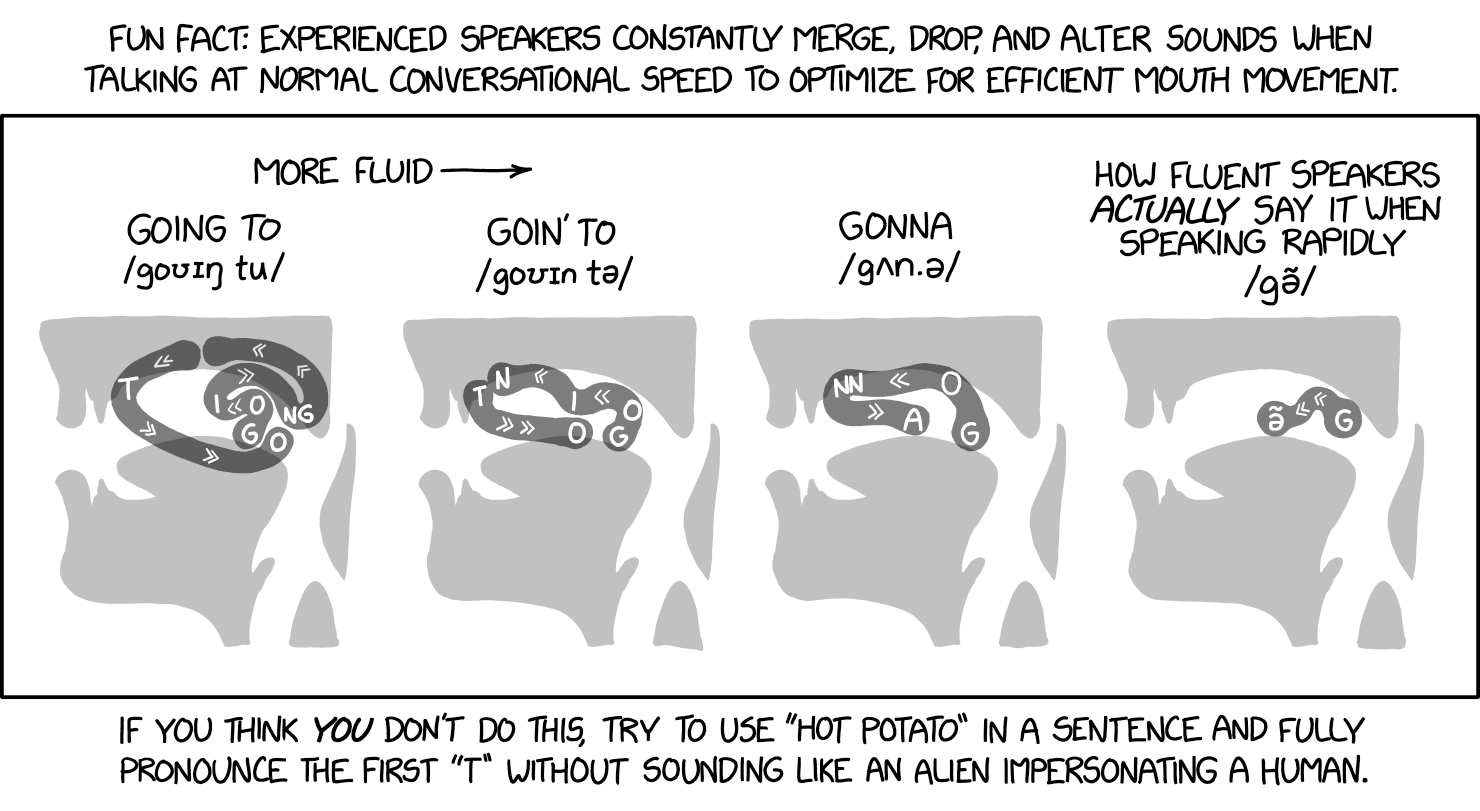
\includegraphics[width=0.8\textwidth]{figures/fluid_speech_2x.png}
    \caption{Illustration of phonetic reduction in the phrase \textit{going to}. The figure humorously shows the progression from the fully articulated form to an extremely reduced form in rapid speech. By Randall Munroe. Source: \texttt{https://xkcd.com/2942/}.}
    \label{fig:phonetic_reduction}
\end{figure}

\textsc{\is{linking}Linking} refers to the way sounds are joined together across word boundaries. In English, like all languages, there's a tendency to ``glue'' words together, to create smooth, continuous transitions rather than choppy, staccato breaks. This can involve linking consonants to vowels (as in \textit{an apple} /ən æpəl/), vowels to vowels (as in \textit{go in} /gəʊ ɪn/), or even consonants to consonants (as in \textit{top piece} /tɒp piːs/).

\textsc{\is{assimilation!in connected speech}Assimilation} is when a sound takes on characteristics of a neighboring sound, becoming more similar to it in place or manner of articulation. This can happen within words (like the /n/ becoming /m/ before /p/ in \textit{input}), but it's especially common across word boundaries. The phrase \textit{ten books} might be pronounced [ˈtʰɛmˈbʊks] because the /n/ assimilates to the bilabial place of articulation of /b/.

\textsc{\is{reduction!in connected speech}Reduction}, as illustrated in Figure \ref{fig:phonetic_reduction}, involves the simplification of sounds, often resulting in the omission or weakening of sounds. This process is particularly prominent in rapid, casual speech. For example, the phrase \textit{going to} might be pronounced as \textit{gonna} /ɡʌnə/, or even further reduced to something approximating /g\~ə/ (where the tilde indicates a nasalized vowel). This reduction process helps in making speech more fluid and less effortful for the speaker, but it can pose significant challenges for language learners who are accustomed to more deliberate, articulated forms of speech.

These processes are not random but follow predictable patterns that can be taught and practiced. Understanding the principles behind linking, assimilation, and reduction helps not only in producing more natural-sounding speech but also in better understanding native speakers, who naturally employ these processes in everyday conversation.\is{connected speech|)}

\section{Conclusion}

Speech isn't just about making individual sounds. It's the result of a chain of articulators, from the lungs to the lips, all coordinated with split-second timing.

English has about 24 \is{consonant!phonemes, number of}consonant phonemes and 14 \is{vowel!phonemes, number of}vowel phonemes (including diphthongs), but these numbers can vary depending on the dialect. Each of these sounds is characterized by specific features like \is{place of articulation}place and \is{manner of articulation}manner of articulation, \is{voicing}voicing, and \is{tongue!position, for vowels}tongue position.

\is{phoneme!as mental category}Phonemes are the mental categories we use to distinguish meaning in language, while \is{allophone!vs phoneme}allophones are the various physical realizations that we perceive as belonging to a given phoneme. This distinction is crucial for understanding both the perceptual and production aspects of pronunciation.

English \is{syllable!structure}syllable structure can be quite complex, allowing for \is{consonant!clusters}consonant clusters that many languages don't permit. This complexity is governed by \is{phonotactics}phonotactic rules specific to English, but all languages have phonotactic rules.

Beyond individual sounds, \is{suprasegmental}suprasegmental features like \is{stress}stress, \is{intonation}intonation, and \is{rhythm}rhythm play a huge role in English pronunciation.

Finally, in speech, sounds don't exist in isolation. They blend and change through processes like \is{linking}linking, \is{assimilation}assimilation, and \is{reduction}reduction. These \is{connected speech!processes}connected-speech phenomena are part of what make any language's pronunciation so distinctive.

%	Linking: How does the phonetic script illustrate linking?
%	Phonotactics: Has there been any mention of the phonotactics of vowels? For example, that /æ/ must be followed by a consonant:  /æt/, /bæt/, */bæ/
%	Suprasegmental: Defined in terms of segments, but segment is unexplained.


\section{Glossary}

\begin{description}
    \item[Allophone] \is{allophone!definition of}A variant of a phoneme that doesn't change meaning in a given language. For example, the aspirated [tʰ] in \textit{top} and unaspirated [t] in \textit{stop} are allophones of /t/ in English.
    
    \item[Assimilation] \is{assimilation}A process in connected speech where a sound becomes more like a neighboring sound. For instance, \textit{ten books} may be pronounced as [tem bʊks].
    
    \item[Coda] \is{coda!definition of}The consonant(s) following the (vowel) nucleus in a syllable. In \textit{cat} /kæt/, /t/ is the coda.
    
    \item[Connected speech] \is{connected speech}The continuous flow of sounds in natural speech, often involving processes that modify individual word pronunciations.
    
    \item[Intonation] \is{intonation}The rise and fall of voice pitch over phrases and sentences, conveying various linguistic and paralinguistic meanings.
    
    \item[Linking] \is{linking}The connection of sounds across word boundaries in connected speech, as in \textit{an apple} [ən æpl].
    
    \item[Nucleus] \is{nucleus (syllable)!definition of}The core of a syllable, typically a vowel. In \textit{cat} /kæt/, /æ/ is the nucleus.
    
    \item[Onset] \is{onset!definition of}The consonant(s) preceding the nucleus in a syllable. In \textit{cat} /kæt/, /k/ is the onset.
    
    \item[Phoneme] \is{phoneme!definition of}The smallest unit of sound that can distinguish meaning in a language. Changing /b/ to /p/ turns \textit{bat} into \textit{pat}.
    
    \item[Phonotactics] \is{phonotactics!definition of}The rules governing possible sound combinations in a language. English allows /sl/ as an onset (e.g., \textit{slide}) but not as a coda.
    
    \item[Reduction] \is{reduction}The weakening or omission of sounds in connected speech, often in unstressed syllables. For example, \textit{going to} may be pronounced as \textit{gonna}.
    
    \item[Rhythm] \is{rhythm}The timing pattern of stressed and unstressed syllables in speech.

    \item[Sibilant] \is{sibilant!definition of}A type of fricative or affricate consonant characterized by a high-pitched hissing sound, produced when air is forced through a narrow channel between the tongue and the roof of the mouth or teeth. In English, sibilants include the fricatives /s/, /z/, /ʃ/ (as in \textit{sh}ip), /ʒ/ (as in mea\textit{s}ure), and the affricates /t͡ʃ/ (as in \textit{ch}ip) and /d͡ʒ/ (as in \textit{j}ump).

    \item[Stress] \is{stress}The relative prominence given to certain syllables or words, through a combination of pitch, length, and loudness.
    
    \item[Suprasegmental] \is{suprasegmental}Features of speech that extend over more than one sound segment, including stress, intonation, and rhythm.
    
    \item[Syllable] \is{syllable}A unit of pronunciation typically consisting of a vowel (nucleus) with optional consonants before (onset) and after (coda).
    
    \item[Voicing] \is{voicing!definition of}The vibration of the vocal cords during the production of a speech sound. Voiced sounds (like /b/, /d/, /g/, /v/, /z/, /ð/ as in \textit{th}is) involve this vibration, while voiceless sounds (like /p/, /t/, /k/, /f/, /s/, /θ/ as in \textit{th}in) do not. Voicing is a key feature distinguishing many consonant pairs in English.
\end{description}

Note: These definitions are simplified for accessibility and may not capture all nuances or exceptions. In practice, many of these concepts have complex interactions and variations across different contexts and varieties of English.